\section{The two galleries in one Schur algebroid}

Write $C_P=C_{w_P}$, $\pi_P=h_P$, $\Pi_n=v^{-\binom n2}[n]_{v^2}!$,
$[n]=\Pi_n/\Pi_{n-1}$, and $\eta=[2]=v+v^{-1}$. For a consecutive
interval $[a,b]$ in a parabolic set we mean $s_a,\ldots,s_b$.
In the right spherical module the sequence of merge targets
$P_1,\ldots,P_d$ represents
\[
 D(P_1,\ldots,P_d)=
 \frac{C_I C_{P_1}\cdots C_{P_d}}
 {\prod_{i=1}^d\pi_{P_{i-1}\cap P_i}},\qquad P_0=I .
\]
Between consecutive targets one splits to their intersection and
merges to the next target. The splits are inclusions. Before inversion
the merge from $X$ to $Y\supset X$ is left multiplication by
$C_Y/\pi_X$ on the appropriate image. Inversion reverses the product.
Thus every quotient below is integral on its specified domain
(A, Lemma 3B.1; B, Definition 3.2 and Lemma 3.3).

\begin{center}
\begin{tabular}{@{}lll@{}}
Symbol & Generators & Position blocks or symmetric-group type\\
\hline
$I$ & $[1,N-1]$ & $(N)$\\
$J$ & $S\setminus\{s_m,s_{m+1}\}$ & $(2m,1)$ across the cut\\
$V$ & $I\cap J$ & $(m,1,m)$\\
$K$ & $[2,N-2]$ & $(1,2m-1,1)$\\
$L$ & $K\cap J=K\cap V$ & $(1,m-1,1,m-1,1)$\\
$K'$ & $I\setminus\{s_1,s_{m+1}\}$ & $(1,m,m)$\\
$E$ & $[3,N-1]$ & $(1,1,2m-1)$\\
$T$ & $J\cap K'=V\cap K'$ & $(1,m-1,1,m)$\\
$D'$ & $E\cap K'$ & $(1,1,m-1,m)$
\end{tabular}
\end{center}

In particular $\R=D(J,K,V)$ and $\BS_m=D(J,K',E)$. Both start with
$F=C_I C_J/\pi_V$; this is itself canonical by B, Lemmas 3.1 and
3.19. The first two stages of our web are
$I\supset V\subset J$. For the general $\BS_j$ replace $J,K'$ by
$J_j=S\setminus\{s_j,s_{j+1}\}$ and $K_j=I\setminus\{s_1,s_{j+1}\}$.
The cut is crossed by merging the final $N-j-1$ packet with the first
$j$ packet; the singleton stays separate. The intermediate splittings
have blocks $(j,1,N-j-1)$, $(1,j-1,1,N-j-1)$, and
$(1,1,j-1,N-j-1)$, apart from the degeneracy at $j=1$, where the
last two overlaps both equal $K_1=E$. For $\CBS_s=D(P_s,E)$,
$P_s=S\setminus\{s_s\}$; one joins the packets $(s,N-s)$ across
the cut, then splits to $(1,1,s-2,N-s)$ and merges the last two
packets, omitting zero packets. These rotations and their inverse
undo one another in determinant degree. Explicitly
$C_{J_j}=\tau^{-(N-j-1)} C_{[1,N-2]}\tau^{N-j-1}$ and
$C_{P_s}=\tau^{-(N-s)} C_I\tau^{N-s}$ (A, Lemma 2C.9).

For $j\ge2$ the three overlaps for $\BS_j$ have factors
$\Pi_j\Pi_{N-j-1}$, $\Pi_{j-1}\Pi_{N-j-1}$,
$\Pi_{j-1}\Pi_{N-j-1}$; for $j=1$ these same scalar formulas hold.
For $\CBS_s$ they are $\Pi_s\Pi_{N-s}$ and $\Pi_{s-2}\Pi_{N-s}$.
Our three factors are $\Pi_m^2,\Pi_{m-1}^2,\Pi_{m-1}^2$.
The length contribution at an individual merge is
$\ell(w_{P_i})-\ell(w_{P_{i-1}\cap P_i})$.

\clearpage
\subsection{An exact identity before canonical correction}

Set $Q_1=[2,m]$, $Q_2=[1,m-1]$ and let $T_1,T_2$ denote right
multiplication by $C_{Q_1}/\Pi_{m-1},C_{Q_2}/\Pi_{m-1}$, respectively,
on the indicated spherical subspaces. Then
\[
 \boxed{\quad\R=D(J,K',E,K',V)=\BS_m T_1T_2.\quad}                 \tag{*}
\]
The maximal moving words in these two normalized parabolic factors
are exactly $s_2\cdots s_m$ and $s_1\cdots s_{m-1}$ from B, Lemma
2.4. The equality holds for the full standard and canonical expansions.

\smallskip
\noindent\textit{Proof.}
Refine $J$ to $V$ in both galleries. The first overlaps are $L\subset V$
and $T\subset V$, so this factors an inclusion. Everything after this
refinement is a finite flag calculation. Fix the two end flags
$U\subset U'$ and $W\subset W'$ of dimensions $m,m+1$ in an
$N$-space over $\mathbb F_q$. In the $V,K,V$ gallery the $K$-flag is
a line $a\subset U\cap W$ and a hyperplane $H\supset U'+W'$.
In the $V,K',E,K',V$ gallery the two $K'$-flags are $(a,U'),(a,W')$,
and the $E$-flag is $(a,D_2)$ with
$a\subset D_2\subset U'\cap W'$, $\dim D_2=2$. All refinements are
uniquely determined by these data. If $d=\dim(U'\cap W')$, then
\[
 \dim((U'\cap W')/a)=d-1=N-\dim(U'+W').
\]
For each $a$, the numbers of two-planes and hyperplanes are therefore
equal. Each gallery counts $[\dim(U\cap W)]_q[d-1]_q$ points, where
$[k]_q=1+\cdots+q^{k-1}$ and $[0]_q=0$.

The normalization shifts agree. Writing $b_n=\binom n2$, the first
tail contributes $b_{2m-1}+2b_m-4b_{m-1}$, and the second contributes
$b_{2m-1}+6b_m-4(b_m+b_{m-1})$. The two galleries have the same input and output flags, so the orbit-dependent standard shifts also agree.
Equality over every finite field gives the generic Schur identity.
Finally $K'=Q_1\times[m+2,N-1]$ and $V=Q_2\times[m+2,N-1]$.
The common factor lies in $E$, commutes with $Q_1,Q_2$, and cancels
one $\Pi_m$ from each of $\pi_{D'}=\pi_T=\Pi_m\Pi_{m-1}$.
This gives $(*)$.\hfill$\square$

\begin{center}
% Needs tikz and xcolor. Read each panel upwards.
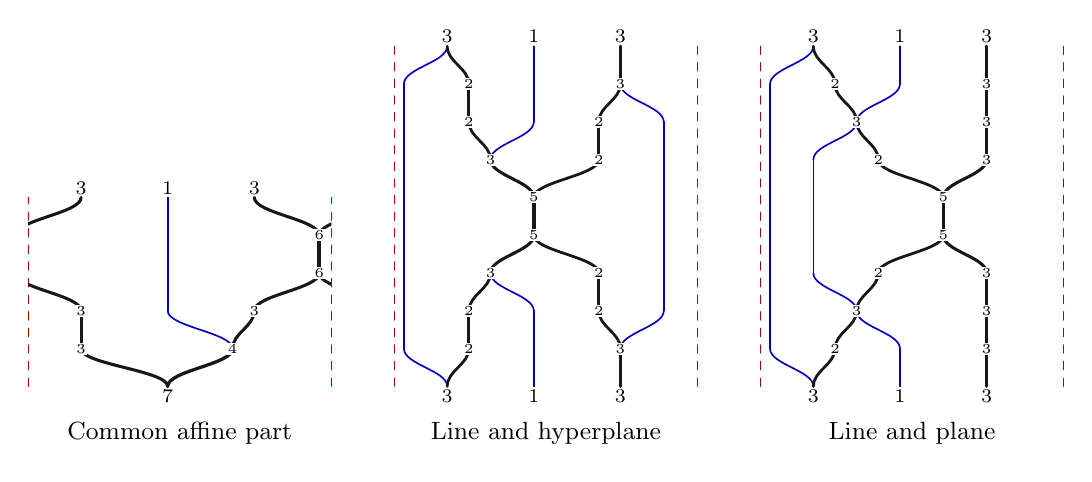
\begin{tikzpicture}[x=.55cm,y=.48cm,line cap=round,line join=round,baseline=(current bounding box.center)]
\begin{scope}[xshift=0cm]
\draw[red!68!black,dashed,thin] (.28,0)--(.28,5) (7.28,0)--(7.28,5);
\begin{scope}\clip (.28,-.18) rectangle (7.28,5.18);
\draw[black!91,line width=1.1042562584220408pt] (3.5,0) .. controls (3.5,0.42) and (1.5,0.58) .. (1.5,1);
\draw[black!91,line width=1.19pt] (3.5,0) .. controls (3.5,0.42) and (5.0,0.58) .. (5.0,1);
\draw[black!91,line width=1.1042562584220408pt] (1.5,1) .. controls (1.5,1.42) and (1.5,1.58) .. (1.5,2);
\draw[blue!74!black,line width=0.6pt] (5.0,1) .. controls (5.0,1.42) and (3.5,1.58) .. (3.5,2);
\draw[black!91,line width=1.1042562584220408pt] (5.0,1) .. controls (5.0,1.42) and (5.5,1.58) .. (5.5,2);
\draw[black!91,line width=1.1042562584220408pt] (1.5,2) .. controls (1.5,2.42) and (0.0,2.58) .. (0.0,3);
\draw[blue!74!black,line width=0.6pt] (3.5,2) .. controls (3.5,2.42) and (3.5,2.58) .. (3.5,3);
\draw[black!91,line width=1.1042562584220408pt] (5.5,2) .. controls (5.5,2.42) and (7.0,2.58) .. (7.0,3);
\draw[black!91,line width=1.1042562584220408pt] (8.5,2) .. controls (8.5,2.42) and (7.0,2.58) .. (7.0,3);
\draw[blue!74!black,line width=0.6pt] (3.5,3) .. controls (3.5,3.42) and (3.5,3.58) .. (3.5,4);
\draw[black!91,line width=1.333836717690617pt] (7.0,3) .. controls (7.0,3.42) and (7.0,3.58) .. (7.0,4);
\draw[black!91,line width=1.1042562584220408pt] (0.0,4) .. controls (0.0,4.42) and (1.5,4.58) .. (1.5,5);
\draw[blue!74!black,line width=0.6pt] (3.5,4) .. controls (3.5,4.42) and (3.5,4.58) .. (3.5,5);
\draw[black!91,line width=1.1042562584220408pt] (7.0,4) .. controls (7.0,4.42) and (5.5,4.58) .. (5.5,5);
\draw[black!91,line width=1.1042562584220408pt] (7.0,4) .. controls (7.0,4.42) and (8.5,4.58) .. (8.5,5);
\end{scope}
\node[fill=white,inner sep=.55pt,font=\tiny] at (1.5,1) {$3$};
\node[fill=white,inner sep=.55pt,font=\tiny] at (5.0,1) {$4$};
\node[fill=white,inner sep=.55pt,font=\tiny] at (1.5,2) {$3$};
\node[fill=white,inner sep=.55pt,font=\tiny] at (5.5,2) {$3$};
\node[fill=white,inner sep=.55pt,font=\tiny] at (7.0,3) {$6$};
\node[fill=white,inner sep=.55pt,font=\tiny] at (7.0,4) {$6$};
\node[below,inner sep=1pt,font=\scriptsize] at (3.5,0) {$7$};
\node[above,inner sep=1pt,font=\scriptsize] at (1.5,5) {$3$};
\node[above,inner sep=1pt,font=\scriptsize] at (3.5,5) {$1$};
\node[above,inner sep=1pt,font=\scriptsize] at (5.5,5) {$3$};
\node[below,align=center,font=\small] at (3.78,-.70) {Common affine part};\end{scope}
\begin{scope}[xshift=4.65cm]
\draw[red!68!black,dashed,thin] (.28,0)--(.28,9) (7.28,0)--(7.28,9);
\begin{scope}\clip (.28,-.18) rectangle (7.28,9.18);
\draw[blue!74!black,line width=0.6pt] (1.5,0) .. controls (1.5,0.42) and (0.5,0.58) .. (0.5,1);
\draw[black!91,line width=1.0025483399593904pt] (1.5,0) .. controls (1.5,0.42) and (2.0,0.58) .. (2.0,1);
\draw[blue!74!black,line width=0.6pt] (3.5,0) .. controls (3.5,0.42) and (3.5,0.58) .. (3.5,1);
\draw[black!91,line width=1.1042562584220408pt] (5.5,0) .. controls (5.5,0.42) and (5.5,0.58) .. (5.5,1);
\draw[blue!74!black,line width=0.6pt] (0.5,1) .. controls (0.5,1.42) and (0.5,1.58) .. (0.5,2);
\draw[black!91,line width=1.0025483399593904pt] (2.0,1) .. controls (2.0,1.42) and (2.0,1.58) .. (2.0,2);
\draw[blue!74!black,line width=0.6pt] (3.5,1) .. controls (3.5,1.42) and (3.5,1.58) .. (3.5,2);
\draw[black!91,line width=1.0025483399593904pt] (5.5,1) .. controls (5.5,1.42) and (5.0,1.58) .. (5.0,2);
\draw[blue!74!black,line width=0.6pt] (5.5,1) .. controls (5.5,1.42) and (6.5,1.58) .. (6.5,2);
\draw[blue!74!black,line width=0.6pt] (0.5,2) .. controls (0.5,2.42) and (0.5,2.58) .. (0.5,3);
\draw[black!91,line width=1.0025483399593904pt] (2.0,2) .. controls (2.0,2.42) and (2.5,2.58) .. (2.5,3);
\draw[blue!74!black,line width=0.6pt] (3.5,2) .. controls (3.5,2.42) and (2.5,2.58) .. (2.5,3);
\draw[black!91,line width=1.0025483399593904pt] (5.0,2) .. controls (5.0,2.42) and (5.0,2.58) .. (5.0,3);
\draw[blue!74!black,line width=0.6pt] (6.5,2) .. controls (6.5,2.42) and (6.5,2.58) .. (6.5,3);
\draw[blue!74!black,line width=0.6pt] (0.5,3) .. controls (0.5,3.42) and (0.5,3.58) .. (0.5,4);
\draw[black!91,line width=1.1042562584220408pt] (2.5,3) .. controls (2.5,3.42) and (3.5,3.58) .. (3.5,4);
\draw[black!91,line width=1.0025483399593904pt] (5.0,3) .. controls (5.0,3.42) and (3.5,3.58) .. (3.5,4);
\draw[blue!74!black,line width=0.6pt] (6.5,3) .. controls (6.5,3.42) and (6.5,3.58) .. (6.5,4);
\draw[blue!74!black,line width=0.6pt] (0.5,4) .. controls (0.5,4.42) and (0.5,4.58) .. (0.5,5);
\draw[black!91,line width=1.2655417527999329pt] (3.5,4) .. controls (3.5,4.42) and (3.5,4.58) .. (3.5,5);
\draw[blue!74!black,line width=0.6pt] (6.5,4) .. controls (6.5,4.42) and (6.5,4.58) .. (6.5,5);
\draw[blue!74!black,line width=0.6pt] (0.5,5) .. controls (0.5,5.42) and (0.5,5.58) .. (0.5,6);
\draw[black!91,line width=1.1042562584220408pt] (3.5,5) .. controls (3.5,5.42) and (2.5,5.58) .. (2.5,6);
\draw[black!91,line width=1.0025483399593904pt] (3.5,5) .. controls (3.5,5.42) and (5.0,5.58) .. (5.0,6);
\draw[blue!74!black,line width=0.6pt] (6.5,5) .. controls (6.5,5.42) and (6.5,5.58) .. (6.5,6);
\draw[blue!74!black,line width=0.6pt] (0.5,6) .. controls (0.5,6.42) and (0.5,6.58) .. (0.5,7);
\draw[black!91,line width=1.0025483399593904pt] (2.5,6) .. controls (2.5,6.42) and (2.0,6.58) .. (2.0,7);
\draw[blue!74!black,line width=0.6pt] (2.5,6) .. controls (2.5,6.42) and (3.5,6.58) .. (3.5,7);
\draw[black!91,line width=1.0025483399593904pt] (5.0,6) .. controls (5.0,6.42) and (5.0,6.58) .. (5.0,7);
\draw[blue!74!black,line width=0.6pt] (6.5,6) .. controls (6.5,6.42) and (6.5,6.58) .. (6.5,7);
\draw[blue!74!black,line width=0.6pt] (0.5,7) .. controls (0.5,7.42) and (0.5,7.58) .. (0.5,8);
\draw[black!91,line width=1.0025483399593904pt] (2.0,7) .. controls (2.0,7.42) and (2.0,7.58) .. (2.0,8);
\draw[blue!74!black,line width=0.6pt] (3.5,7) .. controls (3.5,7.42) and (3.5,7.58) .. (3.5,8);
\draw[black!91,line width=1.0025483399593904pt] (5.0,7) .. controls (5.0,7.42) and (5.5,7.58) .. (5.5,8);
\draw[blue!74!black,line width=0.6pt] (6.5,7) .. controls (6.5,7.42) and (5.5,7.58) .. (5.5,8);
\draw[blue!74!black,line width=0.6pt] (0.5,8) .. controls (0.5,8.42) and (1.5,8.58) .. (1.5,9);
\draw[black!91,line width=1.0025483399593904pt] (2.0,8) .. controls (2.0,8.42) and (1.5,8.58) .. (1.5,9);
\draw[blue!74!black,line width=0.6pt] (3.5,8) .. controls (3.5,8.42) and (3.5,8.58) .. (3.5,9);
\draw[black!91,line width=1.1042562584220408pt] (5.5,8) .. controls (5.5,8.42) and (5.5,8.58) .. (5.5,9);
\end{scope}
\node[fill=white,inner sep=.55pt,font=\tiny] at (2.0,1) {$2$};
\node[fill=white,inner sep=.55pt,font=\tiny] at (5.5,1) {$3$};
\node[fill=white,inner sep=.55pt,font=\tiny] at (2.0,2) {$2$};
\node[fill=white,inner sep=.55pt,font=\tiny] at (5.0,2) {$2$};
\node[fill=white,inner sep=.55pt,font=\tiny] at (2.5,3) {$3$};
\node[fill=white,inner sep=.55pt,font=\tiny] at (5.0,3) {$2$};
\node[fill=white,inner sep=.55pt,font=\tiny] at (3.5,4) {$5$};
\node[fill=white,inner sep=.55pt,font=\tiny] at (3.5,5) {$5$};
\node[fill=white,inner sep=.55pt,font=\tiny] at (2.5,6) {$3$};
\node[fill=white,inner sep=.55pt,font=\tiny] at (5.0,6) {$2$};
\node[fill=white,inner sep=.55pt,font=\tiny] at (2.0,7) {$2$};
\node[fill=white,inner sep=.55pt,font=\tiny] at (5.0,7) {$2$};
\node[fill=white,inner sep=.55pt,font=\tiny] at (2.0,8) {$2$};
\node[fill=white,inner sep=.55pt,font=\tiny] at (5.5,8) {$3$};
\node[below,inner sep=1pt,font=\scriptsize] at (1.5,0) {$3$};
\node[below,inner sep=1pt,font=\scriptsize] at (3.5,0) {$1$};
\node[below,inner sep=1pt,font=\scriptsize] at (5.5,0) {$3$};
\node[above,inner sep=1pt,font=\scriptsize] at (1.5,9) {$3$};
\node[above,inner sep=1pt,font=\scriptsize] at (3.5,9) {$1$};
\node[above,inner sep=1pt,font=\scriptsize] at (5.5,9) {$3$};
\node[below,align=center,font=\small] at (3.78,-.70) {Line and hyperplane};\end{scope}
\begin{scope}[xshift=9.3cm]
\draw[red!68!black,dashed,thin] (.28,0)--(.28,9) (7.28,0)--(7.28,9);
\begin{scope}\clip (.28,-.18) rectangle (7.28,9.18);
\draw[blue!74!black,line width=0.6pt] (1.5,0) .. controls (1.5,0.42) and (0.5,0.58) .. (0.5,1);
\draw[black!91,line width=1.0025483399593904pt] (1.5,0) .. controls (1.5,0.42) and (2.0,0.58) .. (2.0,1);
\draw[blue!74!black,line width=0.6pt] (3.5,0) .. controls (3.5,0.42) and (3.5,0.58) .. (3.5,1);
\draw[black!91,line width=1.1042562584220408pt] (5.5,0) .. controls (5.5,0.42) and (5.5,0.58) .. (5.5,1);
\draw[blue!74!black,line width=0.6pt] (0.5,1) .. controls (0.5,1.42) and (0.5,1.58) .. (0.5,2);
\draw[black!91,line width=1.0025483399593904pt] (2.0,1) .. controls (2.0,1.42) and (2.5,1.58) .. (2.5,2);
\draw[blue!74!black,line width=0.6pt] (3.5,1) .. controls (3.5,1.42) and (2.5,1.58) .. (2.5,2);
\draw[black!91,line width=1.1042562584220408pt] (5.5,1) .. controls (5.5,1.42) and (5.5,1.58) .. (5.5,2);
\draw[blue!74!black,line width=0.6pt] (0.5,2) .. controls (0.5,2.42) and (0.5,2.58) .. (0.5,3);
\draw[blue!74!black,line width=0.6pt] (2.5,2) .. controls (2.5,2.42) and (1.5,2.58) .. (1.5,3);
\draw[black!91,line width=1.0025483399593904pt] (2.5,2) .. controls (2.5,2.42) and (3.0,2.58) .. (3.0,3);
\draw[black!91,line width=1.1042562584220408pt] (5.5,2) .. controls (5.5,2.42) and (5.5,2.58) .. (5.5,3);
\draw[blue!74!black,line width=0.6pt] (0.5,3) .. controls (0.5,3.42) and (0.5,3.58) .. (0.5,4);
\draw[blue!74!black,line width=0.6pt] (1.5,3) .. controls (1.5,3.42) and (1.5,3.58) .. (1.5,4);
\draw[black!91,line width=1.0025483399593904pt] (3.0,3) .. controls (3.0,3.42) and (4.5,3.58) .. (4.5,4);
\draw[black!91,line width=1.1042562584220408pt] (5.5,3) .. controls (5.5,3.42) and (4.5,3.58) .. (4.5,4);
\draw[blue!74!black,line width=0.6pt] (0.5,4) .. controls (0.5,4.42) and (0.5,4.58) .. (0.5,5);
\draw[blue!74!black,line width=0.6pt] (1.5,4) .. controls (1.5,4.42) and (1.5,4.58) .. (1.5,5);
\draw[black!91,line width=1.2655417527999329pt] (4.5,4) .. controls (4.5,4.42) and (4.5,4.58) .. (4.5,5);
\draw[blue!74!black,line width=0.6pt] (0.5,5) .. controls (0.5,5.42) and (0.5,5.58) .. (0.5,6);
\draw[blue!74!black,line width=0.6pt] (1.5,5) .. controls (1.5,5.42) and (1.5,5.58) .. (1.5,6);
\draw[black!91,line width=1.0025483399593904pt] (4.5,5) .. controls (4.5,5.42) and (3.0,5.58) .. (3.0,6);
\draw[black!91,line width=1.1042562584220408pt] (4.5,5) .. controls (4.5,5.42) and (5.5,5.58) .. (5.5,6);
\draw[blue!74!black,line width=0.6pt] (0.5,6) .. controls (0.5,6.42) and (0.5,6.58) .. (0.5,7);
\draw[blue!74!black,line width=0.6pt] (1.5,6) .. controls (1.5,6.42) and (2.5,6.58) .. (2.5,7);
\draw[black!91,line width=1.0025483399593904pt] (3.0,6) .. controls (3.0,6.42) and (2.5,6.58) .. (2.5,7);
\draw[black!91,line width=1.1042562584220408pt] (5.5,6) .. controls (5.5,6.42) and (5.5,6.58) .. (5.5,7);
\draw[blue!74!black,line width=0.6pt] (0.5,7) .. controls (0.5,7.42) and (0.5,7.58) .. (0.5,8);
\draw[black!91,line width=1.0025483399593904pt] (2.5,7) .. controls (2.5,7.42) and (2.0,7.58) .. (2.0,8);
\draw[blue!74!black,line width=0.6pt] (2.5,7) .. controls (2.5,7.42) and (3.5,7.58) .. (3.5,8);
\draw[black!91,line width=1.1042562584220408pt] (5.5,7) .. controls (5.5,7.42) and (5.5,7.58) .. (5.5,8);
\draw[blue!74!black,line width=0.6pt] (0.5,8) .. controls (0.5,8.42) and (1.5,8.58) .. (1.5,9);
\draw[black!91,line width=1.0025483399593904pt] (2.0,8) .. controls (2.0,8.42) and (1.5,8.58) .. (1.5,9);
\draw[blue!74!black,line width=0.6pt] (3.5,8) .. controls (3.5,8.42) and (3.5,8.58) .. (3.5,9);
\draw[black!91,line width=1.1042562584220408pt] (5.5,8) .. controls (5.5,8.42) and (5.5,8.58) .. (5.5,9);
\end{scope}
\node[fill=white,inner sep=.55pt,font=\tiny] at (2.0,1) {$2$};
\node[fill=white,inner sep=.55pt,font=\tiny] at (5.5,1) {$3$};
\node[fill=white,inner sep=.55pt,font=\tiny] at (2.5,2) {$3$};
\node[fill=white,inner sep=.55pt,font=\tiny] at (5.5,2) {$3$};
\node[fill=white,inner sep=.55pt,font=\tiny] at (3.0,3) {$2$};
\node[fill=white,inner sep=.55pt,font=\tiny] at (5.5,3) {$3$};
\node[fill=white,inner sep=.55pt,font=\tiny] at (4.5,4) {$5$};
\node[fill=white,inner sep=.55pt,font=\tiny] at (4.5,5) {$5$};
\node[fill=white,inner sep=.55pt,font=\tiny] at (3.0,6) {$2$};
\node[fill=white,inner sep=.55pt,font=\tiny] at (5.5,6) {$3$};
\node[fill=white,inner sep=.55pt,font=\tiny] at (2.5,7) {$3$};
\node[fill=white,inner sep=.55pt,font=\tiny] at (5.5,7) {$3$};
\node[fill=white,inner sep=.55pt,font=\tiny] at (2.0,8) {$2$};
\node[fill=white,inner sep=.55pt,font=\tiny] at (5.5,8) {$3$};
\node[below,inner sep=1pt,font=\scriptsize] at (1.5,0) {$3$};
\node[below,inner sep=1pt,font=\scriptsize] at (3.5,0) {$1$};
\node[below,inner sep=1pt,font=\scriptsize] at (5.5,0) {$3$};
\node[above,inner sep=1pt,font=\scriptsize] at (1.5,9) {$3$};
\node[above,inner sep=1pt,font=\scriptsize] at (3.5,9) {$1$};
\node[above,inner sep=1pt,font=\scriptsize] at (5.5,9) {$3$};
\node[below,align=center,font=\small] at (3.78,-.70) {Line and plane};\end{scope}
\end{tikzpicture}

\end{center}
{\small Cut-open webs at $m=3$, read upwards. Stack the common part below either tail and identify each pair of red dashed sides. Blue strands have label one. The label-six strand in the common part straddles the cut. The vertices are the normalized splits and merges of A 2D.4.}\par

\noindent The product of the $2m-2$ individual simple KL elements
differs from the normalized completion for $m\ge3$.
At the identity coordinate, multiplication by $T_1T_2$ acts
by $[m]^2$, whereas the individual factors act by $\eta^{2m-2}$
(B, (3.4)). Since $\eps(\BS_m)\ne0$, evaluation at $v=1$ distinguishes
the two products by $m^2\ne4^{m-1}$ for $m\ge3$. Averaging further by
$C_V/\pi_V$ preserves this coordinate. At $m=2$ each parabolic
factor is already one simple KL element, so the raw products agree.

\clearpage
\subsection{Both finite tails are canonical}
\label{sec:finite-tails}

The finite tails can be compared in finite type~A before applying the
common affine prefix. In the finite spherical module $C_V\mathcal H(S_N)$ put
\[
 \mathsf a_m=\frac{C_VC_KC_V}{\pi_L^2},\qquad
 \mathsf b_m=\frac{C_VC_{K'}C_E}
 {\pi_{V\cap K'}\pi_{K'\cap E}}.
\]
The right $V$-eigenrelations of $F=C_IC_J/\pi_V$ define the module map
\[
 \Phi:C_V\mathcal H(S_N)\longrightarrow C_I\mathcal H(W),
 \qquad \Phi(C_Vh)=Fh.
\]
Thus $\Phi(\mathsf a_m)=\mathcal R_m$ and
$\Phi(\mathsf b_m)=\mathcal{BS}_m$, with all normalization factors included.
Both finite tails are single ordinary canonical elements:
\[
 \mathsf a_m=C_{w_A},\qquad
 w_A=w_0w_{\{s_m,s_{m+1}\}},
 \qquad
 \mathsf b_m=C_{w_B},\qquad
 w_B=[m,m+1,N,N-1,\ldots,m+2,m-1,\ldots,1].
\]
Their minimal left $V$-representatives have lengths $m^2+2m-3$
and $m^2-1$, respectively.

\noindent\textit{Proof.}
In the three-letter notation of the parabolic paper, let
$c_0=c_{\mathsf A^m\mathsf B\mathsf C^m}$, with window
$[1-m,\ldots,0,m+1,N+1,\ldots,N+m]$ and length $m^2$.
For $x\in{}^VW_I$, the map
$C_VH_x\mapsto M_{c_0x}$ identifies the finite standard basis with
the type-$m$ standard span. The window formula gives
$\ell(c_0x)=m^2+\ell(x)$, and the equal-letter and unequal-letter
multiplication rules show that it commutes with finite right Hecke
actions (B, Lemmas 3.8--3.9).
The type-$m$ part of $F$ is just $M_{c_0}$ with coefficient one
(B, Lemma 3.19).
Consequently the standard coefficients of the two finite tails are
exactly the type-$m$ coefficients of the two affine products.

At the boundary $m-r=0$, our six-family estimates give coefficient
one at the unique top and strictly positive valuation at every
proper orbit maximum; refinement adds the nonnegative length
deficit (A, Lemmas 4C.2 and 4D.1).
The lowest-exponent table in the parabolic paper at type $m$ has a unique $AB$ orbit
maximum of valuation zero; the $AA$ maxima have valuation one,
and every nonmaximum has an additional positive length deficit
(B, Proposition 3.21). The top coefficient is one in each case.
The two top words are $\mathsf C^{m-1}\mathsf A\mathsf B\mathsf C
\mathsf A^{m-1}$ and $\mathsf A\mathsf B\mathsf C^m\mathsf A^{m-1}$,
which give the displayed finite permutations. Integrality and bar
invariance of the normalized products now identify both tails by
canonical triangularity.\hfill$\square$

Let $L_m=C_{s_2}\cdots C_{s_m}C_{s_1}\cdots C_{s_{m-1}}$.
The corresponding reflection word takes $w_B$ to $w_A$, increasing
length at every step: first it moves $m+1$ past the larger entries,
then it moves $m$ past them. Finite KL multiplication therefore gives
\begin{align*}
 \mathsf b_mL_m
 &=\mathsf a_m+\sum_{z<w_A}d_z(v)C_z,
 &d_z(v)&\in\mathbb N[v,v^{-1}],\\
 \mathcal{BS}_mL_m
 &=\mathcal R_m+\sum_{z<w_A}d_z(v)\Phi(C_z).
\end{align*}
Only finite canonical indices with left $V$-descents occur in the sum.
The top multiplicity is one. This expresses our web as the image of
the top finite canonical summand after the two simple-reflection
chains. Using the normalized completion instead gives the exact
finite identity $\mathsf b_mT_1T_2=\mathsf a_m$.

For $m=3$, the correction has the following form. On the appropriate
spherical domain, the $S_3$ identity
$C_{\{s,t\}}=C_sC_tC_s-C_s$ gives
\[
 \mathcal R_3=\mathcal{BS}_3(C_2C_3-1)(C_1C_2-1),
 \qquad C_i=C_{s_i}.
\]
For $m=2,3,4,5$ the uncorrected finite product
$\mathsf b_mL_m-\mathsf a_m$ has respectively $0,3,10,20$
distinct canonical terms. These are exact finite checks; the
canonical-tail and summand statements above hold for all $m$.


\clearpage
\subsection{What the corrected seed contains}

Write $b_j=u_{j;m}^{-1}$ and let $[\,\C_b\,]$ denote a coefficient
in the spherical canonical basis. For every $1\le j\le m$,
\[
 \boxed{\ [\,\C_{b_j}\,](\C_{X_0}T_1T_2)=\delta_{jm}.\ }          \tag{**}
\]
At the other end of $(*)$, B, Proposition 3.21, also gives
$\BS_m=\sum_{j=1}^m\C_{z(j,1,0)}$. In fact its standards are in
$\mathbb Z[v]$, with constant term $1$ precisely at the $m$ indicated
orbit maxima and zero elsewhere. Subtracting those canonical elements
leaves a bar-invariant vector in $v\mathbb Z[v]\{M_c\}$, hence zero.
Thus $\R=\sum_{j=1}^m\C_{z(j,1,0)}T_1T_2$. In particular $(**)$
and A, Lemma 4I.1, place each off-diagonal family-F term, once, in
\[
 (\BS_m-\C_{X_0})T_1T_2
 =\Big(\BS_{m-1}-\eta\sum_{s=2}^{m-1}\CBS_s\Big)T_1T_2.
\]
Here $\BS_{m-1}$ is taken in the same period $2m+1$.

\smallskip
\noindent\textit{Proof of $(**)$.} For consecutive generators starting at
$s_a$ let $Z_0=Z$, $Z_i=Z C_{[a,a+i-1]}/\Pi_i$; assume $ZH_s=v^{-1}Z$
for $s\in[a+1,a+i-1]$. The left coset representatives are
$g_k=s_a\cdots s_{a+k-1}$, $0\le k\le i$, so that
\[
 Z_i=\sum_{k=0}^i v^{i-k}ZH_{g_k},
 \quad Z_1=ZC_{s_a},\quad
 Z_i=Z_{i-1}C_{s_{a+i-1}}-Z_{i-2}\quad(i\ge2).
\]
The last generator commutes with $g_k$ for $k\le i-2$, giving the
last recurrence. In B, Proposition 2.8, this subtracts the preceding
cover at each step. The remaining terms $\C_e,\C_{\gamma_k}$ are
eigenvectors for every later generator, since the word for $\gamma_k$
is $BC^kB^{N-2k-1}A^k$. Using $[i+1]=\eta[i]-[i-1]$ gives
\[
 \C_{X_0}T_1=\C_{x_{m-1}}+[m-1]\C_e+
             \sum_{k=1}^{m-2}[m-1-k]\C_{\gamma_k}.
\]
The terms after $\C_{x_{m-1}}$ retain the right descent $s_{m+1}$
upon multiplication by $T_2$, as $s_{m+1}$ commutes with $Q_2$.
Applying the same recurrence to B, Proposition 2.11, yields
\[
 \C_{x_{m-1}}T_2=\C_{\beta_m}+\sum_{t=0}^{m-2}[t+1]\mathcal E_t .
\]
Indeed each canonical term of $\mathcal E_t$ is sorted on its first
$m+1$ positions by B, Lemma 4.12(ii) and (4.17)--(4.18). Every
subsequent generator acts by $\eta$, and each such term has right
descent $s_m$. The canonical basis of the right $s$-spherical
subspace consists of the canonical elements with right descent $s$.
The word of $b_j$ is
$C^{j-1}B^{m-j}A\,|\,B\,|\,CB^{m-j}A^{j-1}$.
The adjacent ascents $AB,BC$ give both missing right descents
$s_m,s_{m+1}$ (B, Lemma 4.9). Therefore none of the remainders
contains any $\C_{b_j}$.\hfill$\square$

\smallskip
By B, Proposition 2.6, the identity coordinate of $\C_{X_0}T_1T_2$
has valuation $3-2m$. For $\C_{\beta_m}$ the valuation is one, so the
full vectors differ. Formula $(**)$ isolates the diagonal within family F.
Section~\ref{sec:partialrows} computes the degree-one identity coordinate
of each family-F constituent by completing successive partial sums.
